\documentclass[12pt,a4paper]{scrartcl}
\usepackage[utf8]{inputenc}
\usepackage{mathtools}
\usepackage[english,russian]{babel}
\usepackage{graphicx}
\usepackage{multicol}

\usepackage[left=30mm, top=15mm, right=15mm, bottom=20mm, nohead, footskip=10mm]{geometry} % настройки полей документа

\title{Графики функций}
\author{Darya Tlepbergenova}

\begin{document}

\maketitle

\pagestyle{plain}
\tableofcontents % Вывод содержания

\newpage
\section{Введение}

Функция (обычно обозначается $y = f(x)$) — это соответствие между двумя множествами, при котором каждому элементу одного множества соответствует \textbf{единственный} элемент другого множества.

\begin{figure}[h]
	\centering
	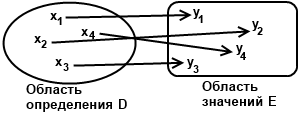
\includegraphics[width=0.5\textwidth]{img/ponyatie-funkcii.png}
	\caption{Понятие функции}
\end{figure}
Допустимые значения аргумента, или \textbf{область определения функции $D(y)$} - это то, что связано с возможными x, при которых функция имеет смысл.

\textbf{Область значений функции $E(y)$} - это то, какие значения принимает y, при допустимых значениях x.

Отсюда следует, что, например, окружность не является функцией.

\begin{figure}[h]
	\centering
	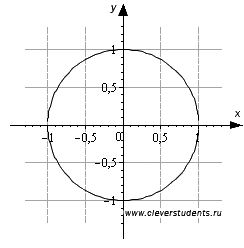
\includegraphics[width=0.3\textwidth]{img/unnamed.png}
	\caption{Здесь одному x (например 0.5) соответствует 2 y}
\end{figure}

\begin{itemize}
    \item x - переменная величина, или, аргумент;
    \item y - зависимая величина – изменяется при изменении аргумента, то есть x согласно какой-либо определенной формуле f, отражающей зависимость одной величины от другой.
\end{itemize}

Далее рассмотрим конструкции элементарных функций.

\newpage
\section{Элементарные функции}

\subsection{Линейная функция $y=kx+b$}
Графиком функции такого вида является прямая. 

\begin{figure}[h!]
	\centering
	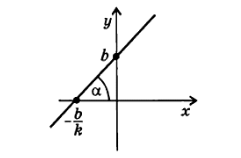
\includegraphics[width=0.4\textwidth]{img/lin.png}
	\caption{Линейная функция}
\end{figure}

Построение делаем с помощью таблицы, достаточно 2 точек (Почему?).

Аналитика параметров функции:

\begin{itemize}
    \item Параметр $b$ - это $f(0) = b$, а значит, точка пересечения с осью OY;
    \item Параметр $k$ - это угловой коэффициент - $k = \tg{\alpha}$ - тангенс угла наклона нашей прямой. Как мы знаем, если $
    \tg{\alpha} > 0 (k > 0)$ то угол $\alpha$ острый, если  $
    \tg{\alpha} < 0 (k < 0)$ то угол $\alpha$ тупой.
\end{itemize}


\subsubsection{Задания}

\begin{figure}[h!]
	\centering
	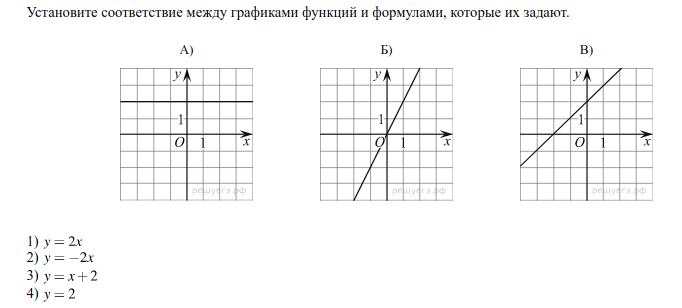
\includegraphics[width=1\textwidth]{img/lin1.png}
\end{figure}

\begin{figure}[h!]
	\centering
	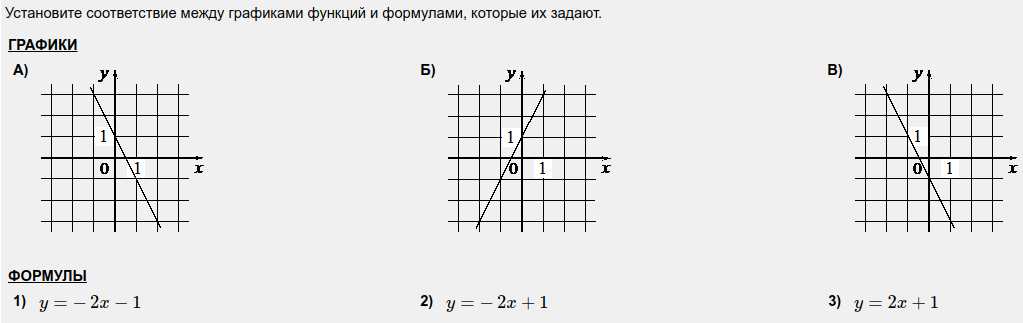
\includegraphics[width=1\textwidth]{img/lin_task2.png}
\end{figure}

\begin{figure}[h!]
	\centering
	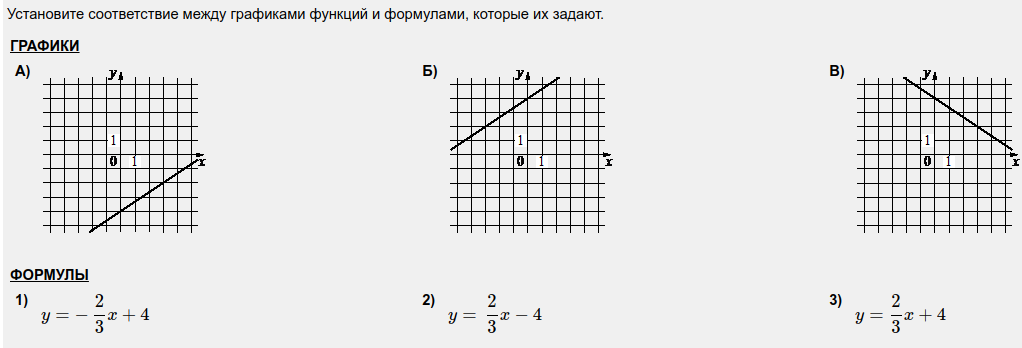
\includegraphics[width=1\textwidth]{img/lin_task3.png}
\end{figure}
\newpage

\subsection{Модуль функции $y=|x|$}
Графиком функции является "галочка".

\begin{figure}[h!]
	\centering
	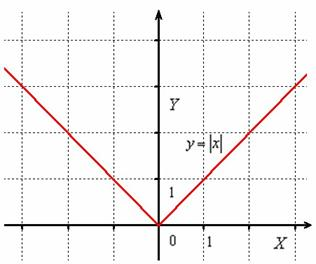
\includegraphics[width=0.5\textwidth]{img/image377.jpg}
	\caption{Функция модуля}
\end{figure}

Перепишем модуль в виде:
\begin{equation*}
    y =
    \begin{cases}
    x, \text{ если } x\geq0 \\
    -x, \text{ если } x<0 \\
    \end{cases}
\end{equation*}

Таким образом, построение сводится к построению линейных функций.

Если под модулем стоит не только x - решается аналогично. Подробнее в разделе Типовые преобразования функций.



\subsection{Функция корня $y= \sqrt{x}$}

Графиком функции такого вида является половинка параболы

(!) Все обратные функции - это поворот вправо на 90 градусов, а так как в действительных числах не существует корня из отрицательного числа - нижняя ветвь параболы отсутствует. Ну и так же, если бы было две ветви - это противоречило бы определению функции - одному x должен соответствовать 1 y.

\begin{figure}[h!]
	\centering
	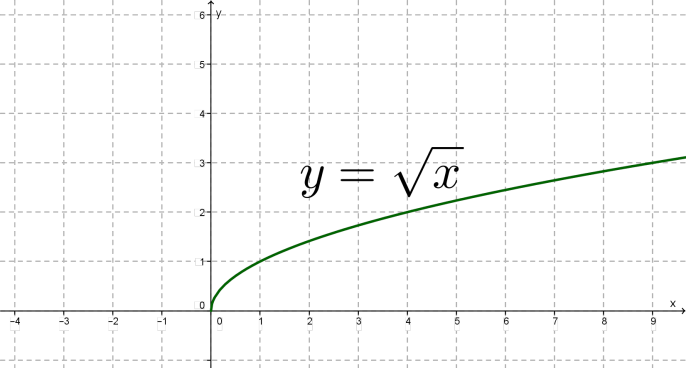
\includegraphics[width=0.5\textwidth]{img/sqrt.png}
	\caption{Функция корня}
\end{figure}

Построение также как и для параболы запоминаем (для простого вида!) точки 1-1 2-4

По точкам, желательно выбирать - 3-4 различных точки для построения.



\subsection{Гипербола $y = \frac{1}{x}$}

У данного графика имеются 2 \textbf{асимптоты} - это прямые к которым график стремится, но никогда не достигает. В данном случае - это OX и OY

\begin{figure}[h!]
	\centering
	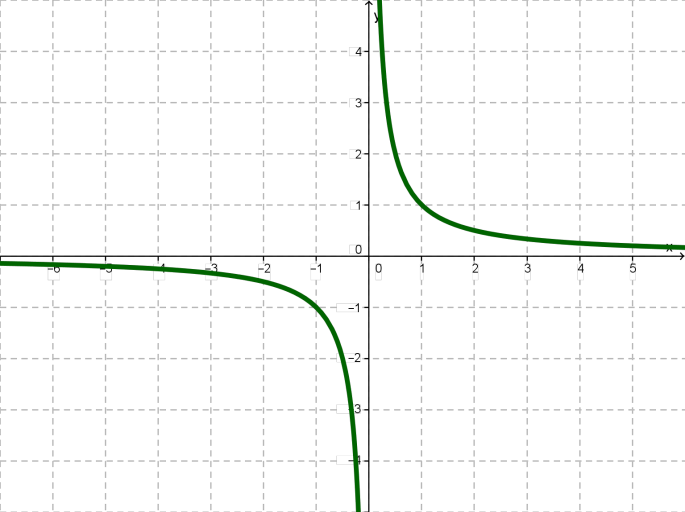
\includegraphics[width=0.7\textwidth]{img/hyp_f.png}
\end{figure}
\newpage

\section{Типовые преобразования элементарных функций}
Обратим внимание сразу, что данные преобразования можно применять к любым функциям. Также мы можем применять сразу несколько преобразований, получая более сложные функции.

\subsection{Преобразование $y = f (x + c)$, c   – число}

Примеры: $y=\sqrt{x+3}$, $y=\frac{1}{x+3}$

\begin{itemize}
    \item В случае $c > 0$ график функции $y = f (x)$ переносится влево на расстояние $|c|$
    \item В случае $c < 0$ график функции $y = f (x)$ переносится вправо на расстояние $|c|$
\end{itemize}

\begin{figure}[h!]
	\begin{minipage}[h]{0.49\linewidth}
		\center{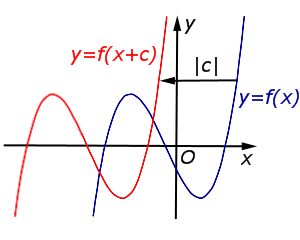
\includegraphics[width=0.7\linewidth]{img/pr1.png} \\ $c > 0$ сдвиг по оси OX влево}
	\end{minipage}
	\hfill
	\begin{minipage}[h]{0.49\linewidth}
		\center{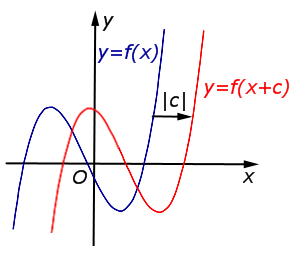
\includegraphics[width=0.7\linewidth]{img/pr2.png} \\ $c < 0$ сдвиг по оси OX вправо}
	\end{minipage}
	\label{ris:image1}
\end{figure}

\subsection{Преобразование $y = f (x) + c$, c   – число}

Примеры: $y=\sqrt{x}+3$, $y=\frac{1}{x}+3$

\begin{itemize}
    \item В случае $c > 0$ график функции $y = f (x)$ переносится вверх на расстояние $|c|$
    \item В случае $c < 0$ график функции $y = f (x)$ переносится вниз на расстояние $|c|$
\end{itemize}

\begin{figure}[h!]
	\begin{minipage}[h]{0.49\linewidth}
		\center{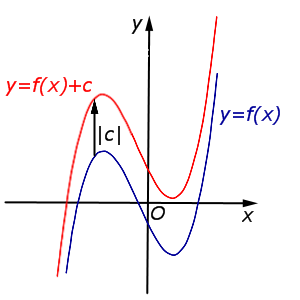
\includegraphics[width=0.7\linewidth]{img/pr3.png} \\ $c > 0$ сдвиг по оси OY вверх}
	\end{minipage}
	\hfill
	\begin{minipage}[h]{0.49\linewidth}
		\center{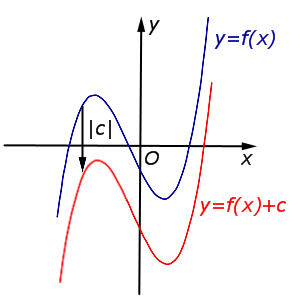
\includegraphics[width=0.7\linewidth]{img/pr4.png} \\ $c < 0$ сдвиг по оси OY вниз}
	\end{minipage}
	\label{ris:image1}
\end{figure}

\subsection{Преобразование отражения  $y = - f(x)$ и $y = f (-x)$}

Примеры: $y=-\sqrt{x}$, $y=\sqrt{-x}$

\begin{itemize}
    \item $y = - f(x)$ \\
    График функции $y = f (x)$ симметрично отражается относительно оси OX.
    \item $y = f (-x)$ \\
    График функции   $y = f (x)$ симметрично отражается относительно оси OY.
\end{itemize}

\begin{figure}[h!]
	\begin{minipage}[h]{0.49\linewidth}
		\center{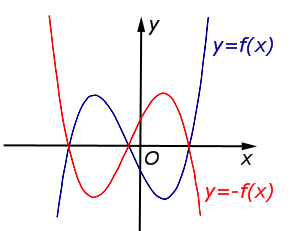
\includegraphics[width=0.7\linewidth]{img/pr5.png} \\ $y = - f(x)$ отражение от OX}
	\end{minipage}
	\hfill
	\begin{minipage}[h]{0.49\linewidth}
		\center{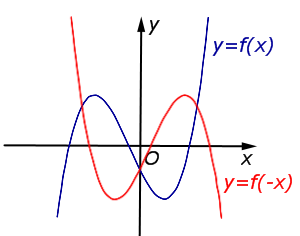
\includegraphics[width=0.7\linewidth]{img/pr6.png} \\ $y = f (-x)$ отражение от OY}
	\end{minipage}
	\label{ris:image1}
\end{figure}

\subsection{Преобразование $y = f (kx)$, k   – число}

Пример: $y=\sqrt{3x}$, $y=\frac{1}{3x}$

\begin{itemize}
    \item В случае $k > 1$ происходит сжатие графика функции $ y = f (x)$ в k раз к оси OY.
    \item В случае   $0 < k < 1$   происходит растяжение графика функции $y = f (x)  $ в  $\frac{1}{|k|}$ раз от оси OY.
\end{itemize}

\begin{figure}[h!]
	\begin{minipage}[h]{0.49\linewidth}
		\center{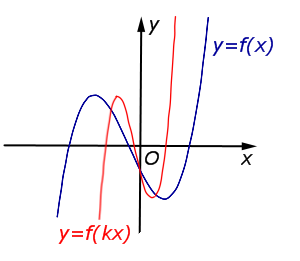
\includegraphics[width=0.7\linewidth]{img/pr7.png} \\ $k > 1$ - сжатие по OX (к OY)}
	\end{minipage}
	\hfill
	\begin{minipage}[h]{0.49\linewidth}
		\center{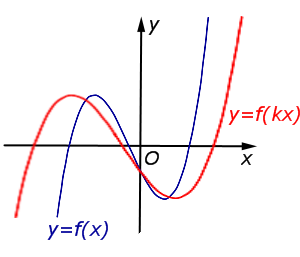
\includegraphics[width=0.7\linewidth]{img/pr8.png} \\ $0 < k < 1$ растяжение по OX (от OY)}
	\end{minipage}
	\label{ris:image1}
\end{figure}

(?) Что будет с графиком при $k<0$? при $-1<k<0$?

\subsection{Преобразование $y = k f (x)$, k   – число}

Пример: $y=3\sqrt{x}$, $y=\frac{3}{x}$

\begin{itemize}
    \item В случае   $k > 1$   происходит растяжение графика функции
    $y = f (x)$ в k раз от оси Ox.
    \item В случае   $0 < k < 1$   происходит сжатие графика функции
    $y = f (x)$ в $\frac{1}{|k|}$ раз к оси Ox.
\end{itemize}

\newpage

\begin{figure}[h!]
	\begin{minipage}[h]{0.49\linewidth}
		\center{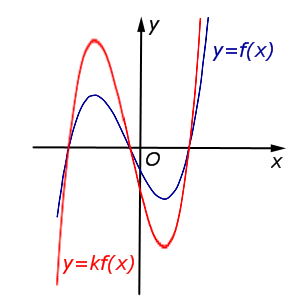
\includegraphics[width=0.7\linewidth]{img/pr11.png} \\ $k > 1$ - растяжение по OY (от OX)}
	\end{minipage}
	\hfill
	\begin{minipage}[h]{0.49\linewidth}
		\center{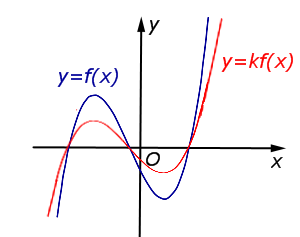
\includegraphics[width=0.9\linewidth]{img/pr12.png} \\ $0 < k < 1$ сжатие по OY (к OX)}
	\end{minipage}
	\label{ris:image1}
\end{figure}

\subsection{Преобразование модуля $y = | f (x)|$ и $y = f (| x|)$}

\begin{itemize}
    \item $y = | f (x)|$. Часть графика функции $y = f (x)$, расположенная в области $y>0$, остаётся на месте. Часть графика функции   y = f (x), расположенная в области $y < 0$, симметрично отражается относительно оси Ox.
    \item $y = f (| x|)$. Ось Oy является осью симметрии
    графика функции   $y = f (| x|)$. Часть графика функции   y = f (x), расположенная в области $x>0$ остаётся на месте. Часть графика функции $y = f (| x|)$, расположенная в области $x < 0$,
    получается из части графика, расположенной в области $x>0$ при помощи симметричного отражения относительно оси Oy.
\end{itemize}

\begin{figure}[h!]
	\begin{minipage}[h]{0.49\linewidth}
		\center{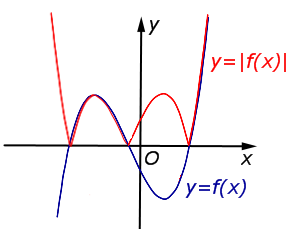
\includegraphics[width=0.7\linewidth]{img/pr15.png} \\ $y = | f (x)|$- отражение от ОХ}
	\end{minipage}
	\hfill
	\begin{minipage}[h]{0.49\linewidth}
		\center{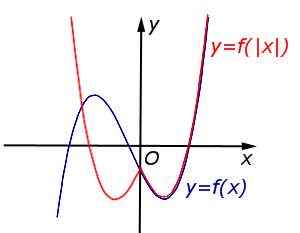
\includegraphics[width=0.7\linewidth]{img/pr16.png} \\ $y = f (| x|)$ отражение от OY}
	\end{minipage}
	\label{ris:image1}
\end{figure}

Пример:
\begin{figure}[h!]
	\begin{minipage}[h]{0.49\linewidth}
		\center{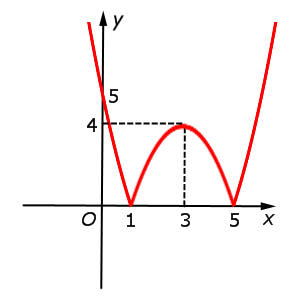
\includegraphics[width=0.6\linewidth]{img/pr_ex1.png} \\ $y = | x^2 - 6x + 5|$}
	\end{minipage}
	\hfill
	\begin{minipage}[h]{0.49\linewidth}
		\center{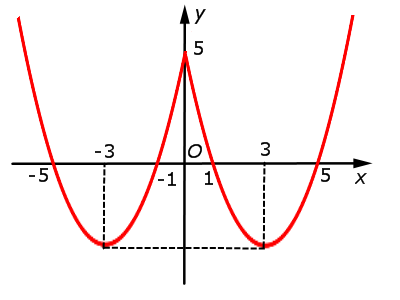
\includegraphics[width=0.65\linewidth]{img/pr_ex2.png} \\ $y = x^2 - 6 |x| + 5$}
	\end{minipage}
	\label{ris:image1}
\end{figure}


\subsection{Задания}

\begin{figure}[h!]
	\centering
	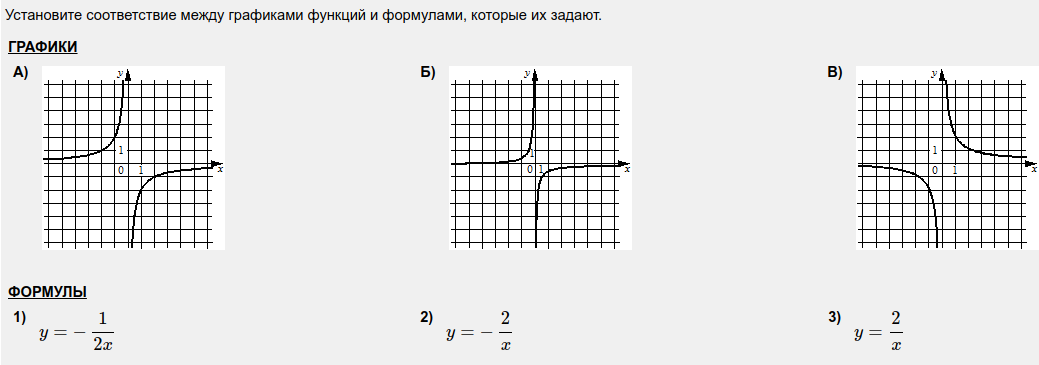
\includegraphics[width=1\textwidth]{img/preobr_t1.png}
\end{figure}

\begin{figure}[h!]
	\centering
	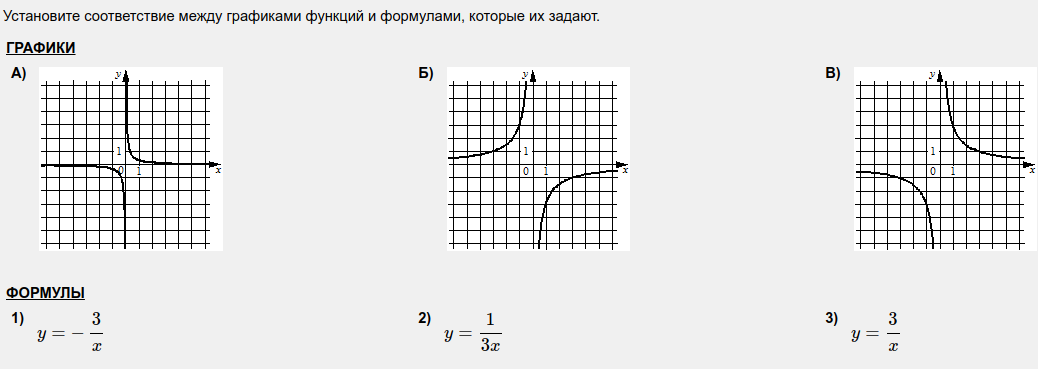
\includegraphics[width=1\textwidth]{img/preobr_t2.png}
\end{figure}

\begin{figure}[h!]
	\centering
	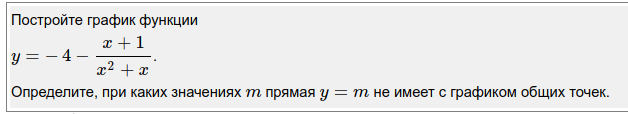
\includegraphics[width=0.9\textwidth]{img/preobr_t3.png}
\end{figure}

\begin{figure}[h!]
	\centering
	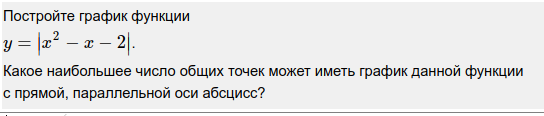
\includegraphics[width=0.9\textwidth]{img/preobr_t4.png}
\end{figure}

\begin{figure}[h!]
	\centering
	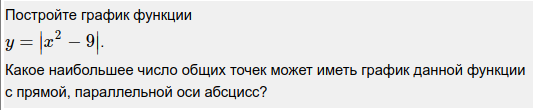
\includegraphics[width=0.9\textwidth]{img/preobr_t5.png}
\end{figure}

\newpage

\section{Элементарные функции (продолжение)}
\subsection{Квадратная функция $y=x^2$}
Графиком функции такого вида является парабола.

\begin{figure}[h!]
	\centering
	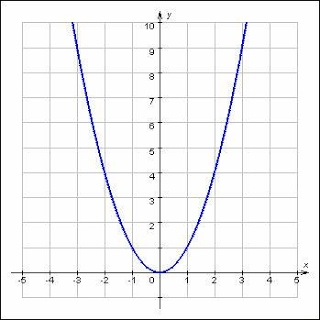
\includegraphics[width=0.5\textwidth]{img/par.jpg}
	\caption{Парабола}
\end{figure}

Общий вид параболы как мы знаем $y = ax^2 + bx + c$. Как мы разбирали в прошлой главе - это преобразования. Для определения конкретного преобразования используют прием - выделение полного квадрата:

\[
    x^2 + 2x - 5 = (x^2 +2x + 1) - 6 = (x + 1)^2 - 6
\]

И теперь видно, что это сдвиг элементарной функции $x^2$ по оси OX влево на 1 и сдвиг вниз по OY на 6.

Также для построения параболы удобно использовать формулу вершины параболы:

\[
    x_0 = -\frac{b}{2a} \text{, } y_0 = f(x_0)
\]

Аналитика функции относительно параметров a,b и c в $y = ax^2 + bx + c$:
\begin{itemize}
    \item Параметр c. Как и, например, в линейной функции b, это свободный член (без x), а значит что это в точности - пересечение графика с осью OY.
    \item Параметр a. как изучали в преобразованиях - это отражение относительно OX. Таким образом, положительное a - ветви вверх, отрицательное - ветви вниз.
    \item Параметр b. Данный параметр участвует в вершине параболы, а значит относительно знака b и a можно понять с какой стороны вершина параболы.
\end{itemize}

Также в построении графика можно использовать корни квадратного уравнения - это будут точки пересечения графика с осью OX.

\[
    x_{1,2} = \frac{-b \pm \sqrt{b^2 - 4ac}}{2a}
\]

\subsubsection{Задания}

\begin{figure}[h!]
	\centering
	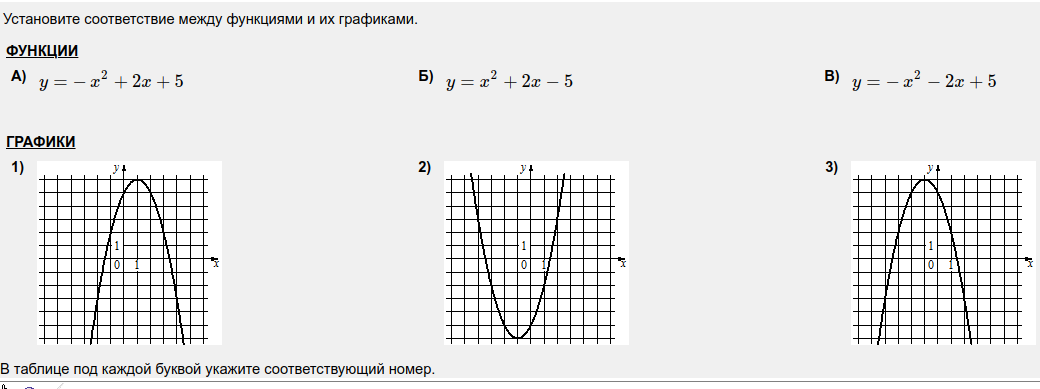
\includegraphics[width=1\textwidth]{img/parab_t1.png}
\end{figure}

\begin{figure}[h!]
	\centering
	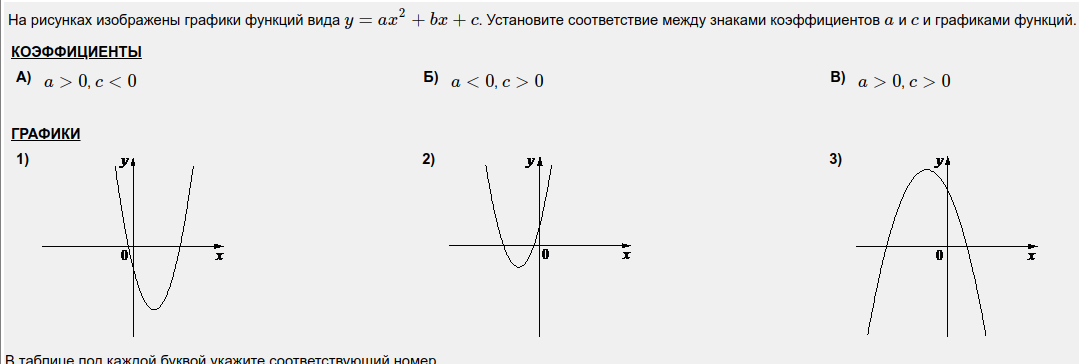
\includegraphics[width=1\textwidth]{img/parab_t2.png}
\end{figure}

\begin{figure}[h!]
	\centering
	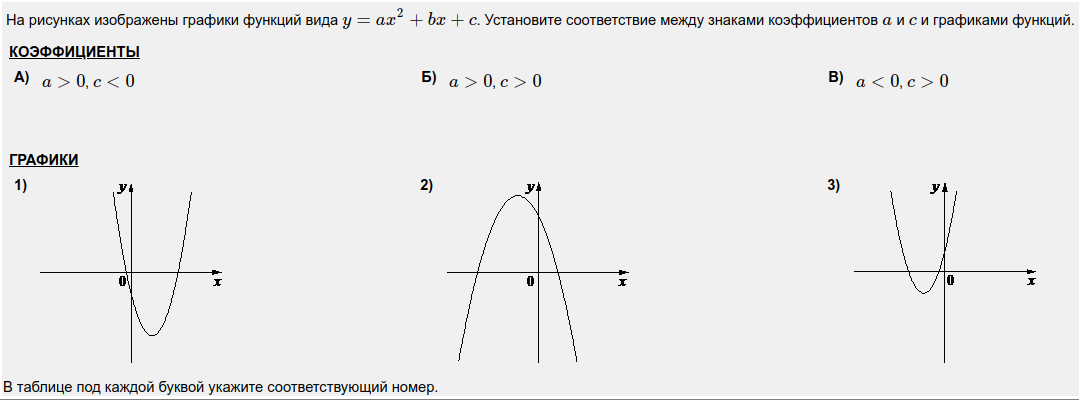
\includegraphics[width=1\textwidth]{img/parab_t3.png}
\end{figure}

\begin{figure}[h!]
	\centering
	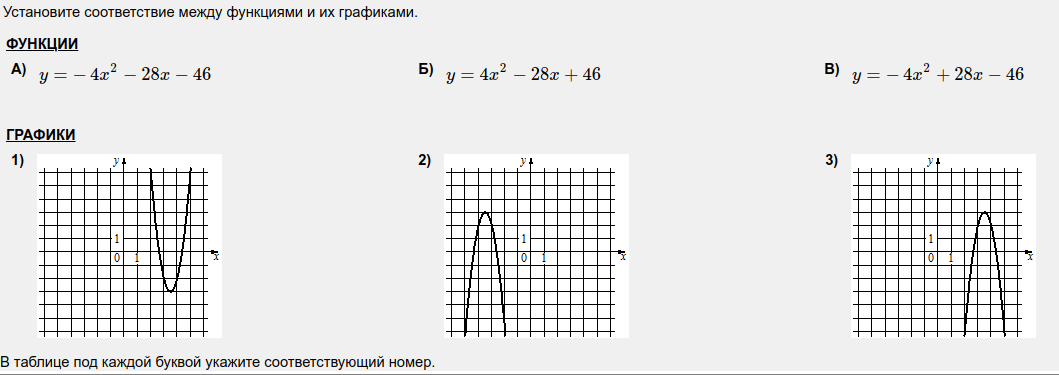
\includegraphics[width=1\textwidth]{img/parab_t4.png}
\end{figure}

\newpage

\subsection{Кубическая функция $y=x^3$}
Графиком функции такого вида является справа от OY - подобная параболе ветка, слева  - такая же только идущая вниз. График является симметричным относительно центра координат.

Фигура называется симметричной относительно точки О, если для каждой точки фигуры симметричная ей точка относительно точки О также принадлежит этой фигуре. Точка О называется центром симметрии фигуры.

\begin{figure}[h!]
	\centering
	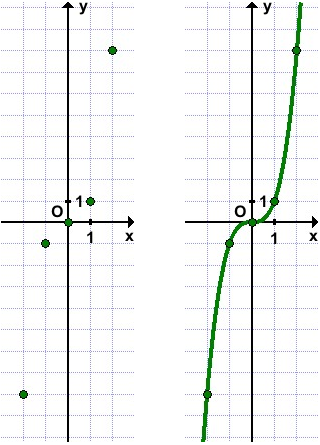
\includegraphics[width=0.5\textwidth]{img/kub.png}
	\caption{Кубическая функция}
\end{figure}

В общем виде: $y = ax^3+bx^2+cx + d$ - поступаем аналогично параболе.

(?) Как строится график функции $y = \sqrt[3]{x}$?

\newpage
\section{Элементарные (посложнее) функции}
\subsection{Тригонометрические функции}
Тригонометрические функции представляют собой элементарные функции, аргументом которых является угол. С помощью тригонометрических функций описываются соотношения между сторонами и острыми углами в прямоугольном треугольнике. 

Для построения функций - необходимо вспомнить единичную окружность на которой мы изображали углы и откладывали косинусы и синусы (другое занятие).

\begin{itemize}
    \item Функция синуса $y = \sin{x}$
    
    \begin{figure}[h!]
	\centering
	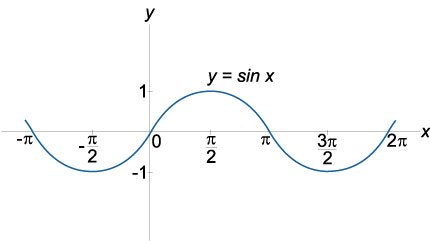
\includegraphics[width=0.5\textwidth]{img/sin.jpg}
    \end{figure}
    
    \item Функция косинуса $y = \cos{x}$
    
    \begin{figure}[h!]
	\centering
	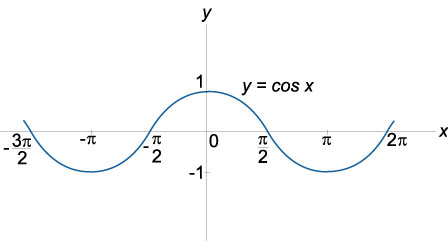
\includegraphics[width=0.5\textwidth]{img/cos.jpg}
    \end{figure}
    
    \item функция тангенса $y = \tg{x}$
    
    \begin{figure}[h!]
	\centering
	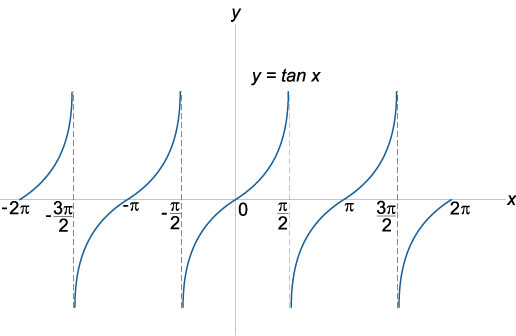
\includegraphics[width=0.5\textwidth]{img/tg.jpg}
    \end{figure}
    
    \item Функция котангенса $y = \ctg{x}$
    
\end{itemize}

\begin{figure}[h!]
\centering
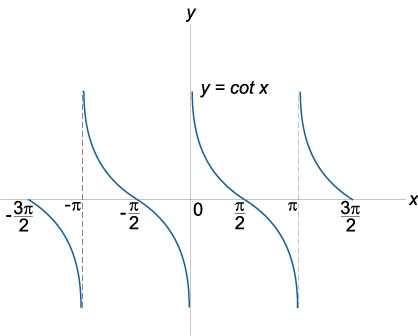
\includegraphics[width=0.5\textwidth]{img/ctg.jpg}
\end{figure}
    
\newpage
Все преобразования, которые мы разбирали здесь также актуальны:

    \begin{figure}[h!]
	\centering
	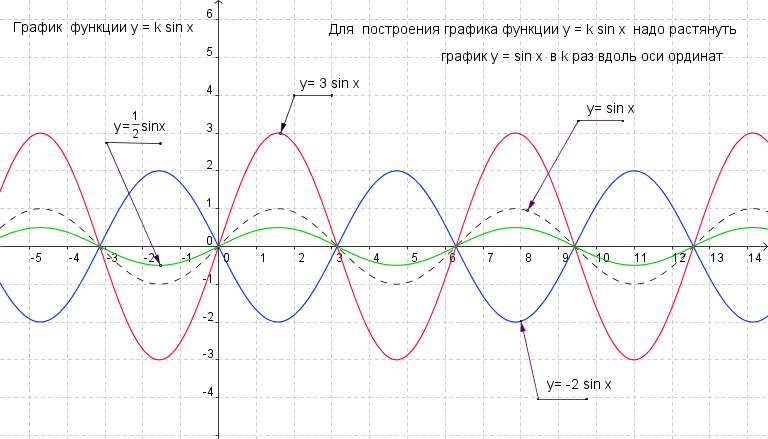
\includegraphics[width=1\textwidth]{img/pr_sin.png}
    \end{figure}

\subsubsection{Задания}

\begin{figure}[h!]
	\centering
	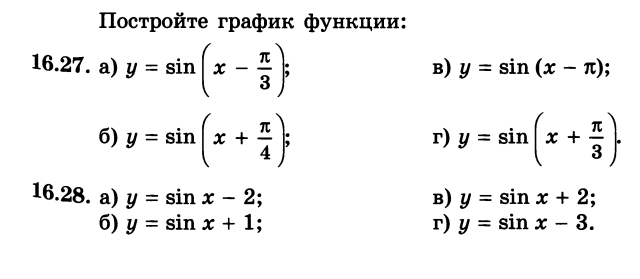
\includegraphics[width=0.7\textwidth]{img/sin_t1.png}
\end{figure}

\begin{figure}[h!]
	\centering
	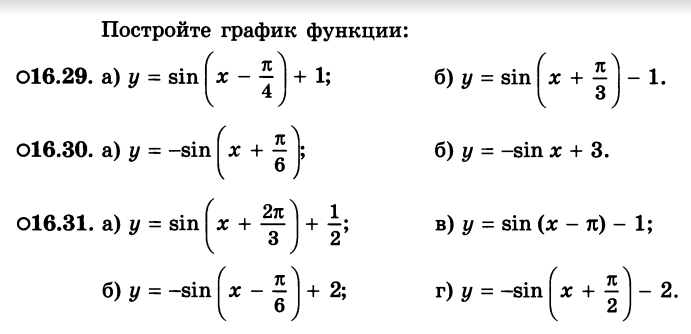
\includegraphics[width=0.7\textwidth]{img/sin_t2.png}
\end{figure}

\begin{figure}[h!]
	\centering
	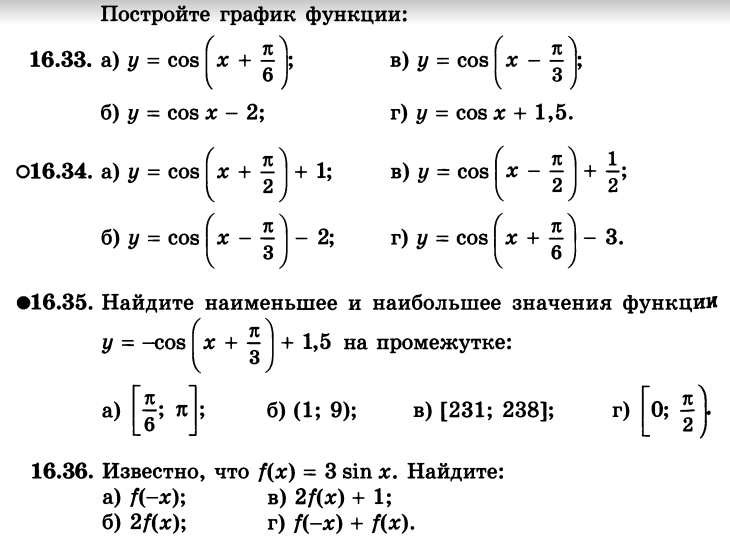
\includegraphics[width=0.7\textwidth]{img/cos_t1.png}
\end{figure}

\begin{figure}[h!]
	\centering
	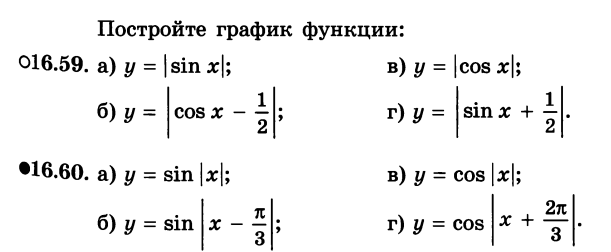
\includegraphics[width=0.7\textwidth]{img/cos_t2.png}
\end{figure}
\newpage
\begin{figure}[h!]
	\centering
	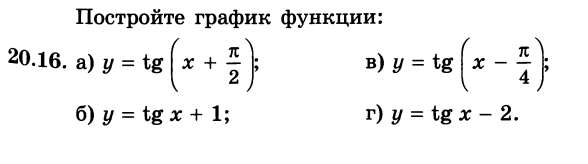
\includegraphics[width=0.7\textwidth]{img/tg_t1.png}
\end{figure}

\newpage

\begin{figure}[h!]
	\centering
	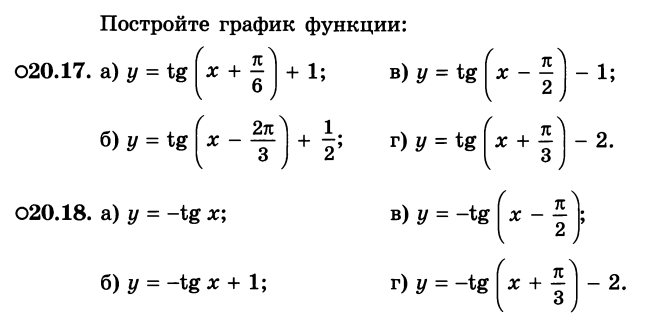
\includegraphics[width=0.7\textwidth]{img/tg_t2.png}
\end{figure}

\begin{figure}[h!]
	\centering
	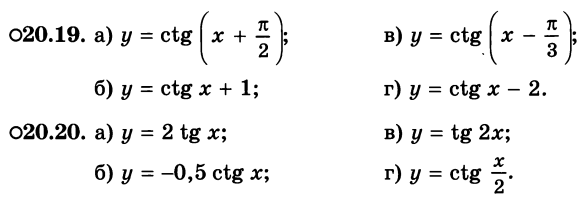
\includegraphics[width=0.7\textwidth]{img/ctg_t1.png}
\end{figure}

\begin{figure}[h!]
	\centering
	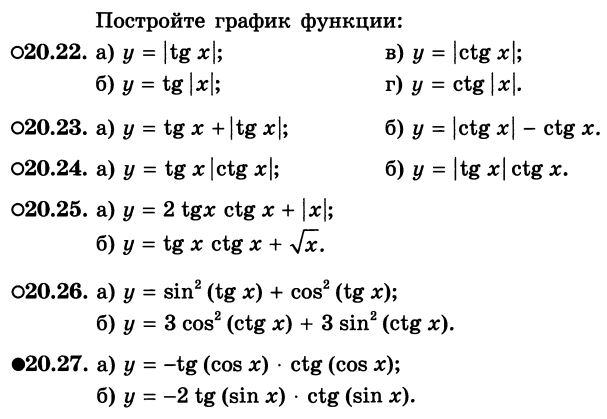
\includegraphics[width=0.7\textwidth]{img/ctg_t2.png}
\end{figure}

\newpage

\subsection{Обратные тригонометрические функции}
Как мы уже говорили - обратные функции - это исходные повернутые на 90 градусов. В силу периодичности тригонометрических функций (также как было с параболой) - нарушается определение функции. По этому принято брать часть этих функций.  Например, у функции 
$y = \arcsin{x}$ область значений рассматривается лишь в промежутке $x \in [-\frac{\pi}{2},\frac{\pi}{2}]$

\begin{itemize}
    \item Арксинус $y = \arcsin{x}$. 
    \begin{figure}[h!]
    \centering
    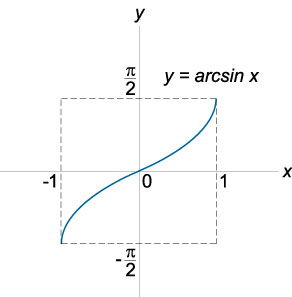
\includegraphics[width=0.5\textwidth]{img/arcsin.jpg}
    \end{figure}
    \item Арккосинус $y = \arccos{x}$
    \begin{figure}[h!]
    \centering
    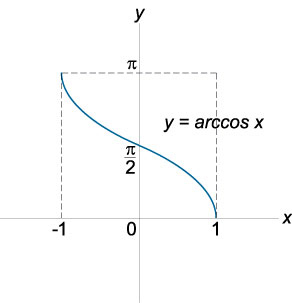
\includegraphics[width=0.5\textwidth]{img/arccos.jpg}
    \end{figure}
    \newpage
    \item Арктангенс $y = \arctg{x}$
    \begin{figure}[h!]
    \centering
    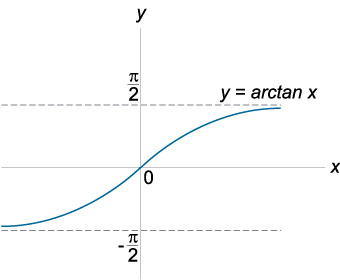
\includegraphics[width=0.5\textwidth]{img/arctg.jpg}
    \end{figure}
    \item Арккотангенс $y = \arcctg{x}$
    \begin{figure}[h!]
    \centering
    \includegraphics[width=0.5\textwidth]{img/arcctg.jpg}
    \end{figure}
\end{itemize}

(?) Какие D(y) и E(y) у представленных выше функций?

\newpage
\subsubsection{Задания}

\begin{figure}[h!]
	\centering
	\includegraphics[width=0.7\textwidth]{img/arcsin_t1.png}
\end{figure}

\begin{figure}[h!]
	\centering
	\includegraphics[width=0.7\textwidth]{img/arccos_t1.png}
\end{figure}

\begin{figure}[h!]
	\centering
	\includegraphics[width=0.7\textwidth]{img/acctg_t1.png}
\end{figure}

\newpage
\subsection{Показательная функция $y = a^x$, где a - число}
Показательная функция - это монотонно возрастающая функция при $a>0$ и монотонно убывающая при $0<a<1$. Именно этим свойством мы пользуемся при решении уравнений и неравенств. (Как именно?)

\begin{figure}[h!]
	\centering
	\includegraphics[width=0.7\textwidth]{img/pokaz.jpg}
	\caption{Показательная функция}
\end{figure}

\subsubsection{Задания}

\begin{figure}[h!]
	\centering
	\includegraphics[width=0.7\textwidth]{img/pokaz_t1.png}
\end{figure}

\begin{figure}[h!]
	\centering
	\includegraphics[width=0.7\textwidth]{img/pokaz_t2.png}
\end{figure}

\newpage
\subsection{Логарифмическая функция $y = \log_a{x}$, где a - число}
Так как логарифм - обратная функция от показательной, она логично получается поворотом на 90 градусов вправо и также делится на 2 случая, относительно параметра a.

\begin{figure}[h!]
	\centering
	\includegraphics[width=0.6\textwidth]{img/log.jpg}
	\caption{Логарифмическая функция}
\end{figure}

\subsubsection{Задания}

\begin{figure}[h!]
	\centering
	\includegraphics[width=0.7\textwidth]{img/log_t1.png}
\end{figure}

\begin{figure}[h!]
	\centering
	\includegraphics[width=0.7\textwidth]{img/log_t2.png}
\end{figure}

\newpage
\section{Что делать с не элементарными функциями?}
Полное описание функции состоит из (то, как строят сложные функции):
\begin{enumerate}
    \item Нахождение области определения функции $D(y)$
    \item Четноть, нечетность, периодичность \\
    Функция называется \textbf{чётной}, если справедливо равенство
    $\displaystyle f(-x) = f(x)$, (график её симметричен относительно центра координат). \\
    Функция называется \textbf{нечётной}, если справедливо равенство
    $\displaystyle f(-x)=-f(x)$, (график её симметричен относительно оси ординат) \\
    \textbf{Ни чётная, ни нечётная функция} такие тоже бывают :) \\
    \textbf{Периодическая функция} ― функция, повторяющая свои значения через некоторый регулярный интервал аргумента, то есть не меняющая своего значения при добавлении к аргументу некоторого фиксированного ненулевого числа (периода функции) на всей области определения. 
    \item Непрерывность
    \item Асимптоты \\
    \textbf{Асимптота} - прямая, обладающая тем свойством, что расстояние от точки кривой до этой прямой стремится к нулю при удалении точки вдоль ветви в бесконечность. \\
    По простому - то, к чему функция стремится, но не может достичь
    \item Нули функции и интервалы знакопостоянства
    \item Интервалы монотонности и экстремумы \\
    \textbf{Монотонность} - возрастание/убывание функции; \\
    \textbf{Экстремум} - максимальное или минимальное значение функции на заданном множестве (то есть на границах не может быть экстремума!). Точка, в которой достигается экстремум, называется точкой экстремума
    \item Выпуклость. Вогнутость. Точка перегиба
    \item Дополнительные точки
    \item Область значений функции $E(y)$
    \item График функции
\end{enumerate}

Пример полного описания функции будет в конце (Приложение 1) 

\subsection{Задание}
Провести полное исследование функции и построить график функции:

\[
    y = \frac{x^2}{4(x+2)}
\]

\newpage
\section*{Приложение 1: Пример полного описания функции} \label{full}
\addcontentsline{toc}{section}{Приложение 1: Пример полного описания функции}

Провести полное исследование функции и построить график функции:

\[
    y = \frac{x^4}{(x+1)^3}
\]

1. Найдем область определения функции: $D(x) = (- \infty,-1) \cup (-1, + \infty)$

2. Четноть, нечетность, периодичность.

Четность: проверим $y(-x) = \frac{x^4}{(-x+1)^3}$, то есть $y(-x) \neq y(x)$. Значит функция не четна.
Нечетность: так как $y(-x) \neq -y(x)$ функция не нечетна.
Так как в состав функции не входят периодичные функции - функция непериодична.

3. Непрерывность: 
Функция элементарная, значит непрерывна на своей области определения, осталось проверить характер разрыва в точке -1:
\[
    \lim_{x \rightarrow -1-0}y(x) = \frac{1}{-0^3} = - \infty 
\]
\[
    \lim_{x \rightarrow -1+0}y(x) = \frac{1}{+0^3} = + \infty 
\]

Значит, -1 - точка разрыва второго рода.

4. Асимптоты: 
Так как при $x = -1$ функция терпит разрыв второго рода, прямая $x = -1$ является вертикальной асимптотой.

Найдем наклонные асимптоты: пусть она имеет вид: $y = kx +b$, тогда

\[
    k = \lim_{x \rightarrow \infty}\frac{x^4}{x \cdot (x+1)^3} = 1
\]

\[
`   b = \lim_{x \rightarrow \infty}(f(x) - kx) = \lim_{x \rightarrow \infty}(\frac{x^4}{(x+1)^3} - x) = \lim_{x \rightarrow \infty}\frac{x^4 - x(x+1)^3}{(x+1)^3} = 
\]
\[
    = \lim_{x \rightarrow \infty} \frac{x^4 - x^4 - 3x^3 - 9x^2 - 27x}{(x + 1)^3} = \lim_{x \rightarrow \infty} \frac{- 3 - \frac{9}{x} - \frac{27}{x^2}}{1 + \frac{9}{x} + \frac{27}{x^2}+\frac{27}{x^3}} = -3
\]

Получили наклонную асимптоту: $y = x - 3$

5. Нули функции и интервалы знакопостоянства.

Данная функция обращается в 0 при $x = 0$. Разобьем числовую прямую на интервалы точками $0$ и $-1$:

\begin{table}[h]
\begin{tabular}{|l|l|l|l|}
\hline
Интервалы    & $(-\infty, -1)$ & $(-1,0)$ & $(0,+\infty)$ \\ \hline
Знак функции & -               & +        & +             \\ \hline
\end{tabular}
\end{table}

Таким образом, функция отрицательна на интервале $(-\infty, -1)$ и положительна на интервале $(-1,0) \cup (0, + \infty)$.

6. Интервалы монотонности и экстремумы.
Найдем стационарные точки:

\[
    y' = \frac{4x^3(x+1)^3 - 3x^4(x+1)^2}{(x+1)^6} = \frac{(x+1)^2 \cdot (4x^4 + 4x^3 - 3x^4)}{(x+1)^6} = 
\]
\[
    =\frac{(x+1)^2 \cdot(x^4 + 4x^3)}{(x+1)^6} = \frac{x^3 \cdot (x+1)^2 \cdot (x+4)}{(x+1)^6} = \frac{x^3(x+4)}{(x+1)^4}
\]

Таким образом, точки подозрительные на экстремум: $0, -1, -4$
Разобьем всю числовую прямую на интервалы этими точками и определим знак производной на этих промежутках для определения характера монотонности функции:

\begin{table}[h]
\begin{tabular}{|l|l|l|l|l|l|l|l|}
\hline
Интервалы & $(- \infty, -4)$ & -4                & (-4,-1) & -1            & (-1,0)  & 0 & $(0,+\infty)$ \\ \hline
$y'(x)$   & +                & 0                 & -       & не существует & -       & 0 & +                          \\ \hline
$y(x)$    & возрастает       & $-\frac{256}{27}$ & убывает & не существует & убывает & 0 & возрастает                 \\ \hline
\end{tabular}
\end{table}

Таким образом, функция возрастает на интервалах $(-\infty,-4) \cup (0,+\infty)$ и убывает на промежутках: $(-4,-1) \cup (-1,0)$. 

Локальный минимум функции: $y(0) = 0$,

Локальный максимум функции: $y(-4) = -\frac{256}{7}$

7. Выпуклость. Вогнутость. Точка перегиба.

Найдем точки перегиба, для этого найдем 2 производную:
\[
    y'' = \left( \frac{x^3(x+4)}{(x+1)^4} \right)' = \frac{(3x^2(x+4)+x^3)\cdot (x+1)^4 - 4(x+1)^3x^3(x+4)}{(x+1)^8} = 
\]
\[
    = \frac{x^2 (x+1)^3\cdot ((3x + 12 + x)(x+1)-4x(x+4))}{(x+1)^8} = 
\]
\[
    =\frac{x^2\cdot4\cdot(x^2+x+3x+3-x^2-4x)}{(x+1)^5} =\frac{12x^2}{(x+1)^5}
\]

Таким образом, точки, подозрительные на перегиб $x=0,-1$

Исследуем выпуклость/вогнутость функции слева и справа от точки разрыва. Для этого нужно определить интервалы знакопостоянства 2 производной:

\begin{table}[h]
\begin{tabular}{|l|l|l|l|l|l|}
\hline
Интервалы & $(-\infty,-1)$ & -1            & $(-1,0)$ & 0 & $(0,+\infty)$ \\ \hline
$y''(x)$  & -              & не существует & +        & 0 & +             \\ \hline
$y(x)$    & выпукла        & не существует & вогнута  & 0 & вогнута       \\ \hline
\end{tabular}
\end{table}

8. Дополнительные точки.

\begin{table}[h]
\begin{tabular}{|l|l|l|l|l|}
\hline
x & 1             & 2               & -2  & 1.5   \\ \hline
y & $\frac{1}{8}$ & $\frac{16}{27}$ & -16 & 0.324 \\ \hline
\end{tabular}
\end{table}

9. Область значений: $E(y) = (- \infty, -\frac{256}{27}) \cup (0, +\infty)$

10. График функции: 

\begin{figure*}[h!]
    \centering
    \includegraphics[width=10cm]{img/graf_var4.png}
\end{figure*}

На графике красным обозначена сама функция, а зеленым и синим ее асимптоты.
\end{document}
